\documentclass[fleqn,parskip=half]{scrbook} % <= Druckversion: "scrbook" / Bildschirmversion: "scrreprt"
\usepackage[ngerman,biber]{hpi-praeambel} % <= Sprache der Arbeit ("ngerman"/"english"), Biblatex-Backend ("bibtex"/"biber")

% ABOUT
% anpassen hpi-praeambel.sty und meta.tex
\newcommand{\hpitype}{\LaTeX}
\newcommand{\hpiauthor}{Jan Unger}
\newcommand{\hpititle}{Python Notizen}
\newcommand{\hpititleother}{} % <= Untertitel
\newcommand{\hpidate}{\today}


% Eingabe anpassen
% Quelle Literaturverzeichnis oder URL in Fussnote 
%\newcommand{\quelle}{\quelle}{Jan Schaffranek franneck94~\footnote{\url{https://github.com/franneck94}}}
%\newcommand{\quelle}{MathePeter siehe~\textcite{peter:2021:mathe}}% Literaturverzeichnis
\newcommand{\titel}{Python Notizen}
\newcommand{\autor}{Jan Unger}
\newcommand{\datum}{\today}
\newcommand{\datumHand}{09.07.2021}% ##.##.####
\newcommand{\website}{http://bw-ju.de}
\newcommand{\websiteKurz}{bw-ju.de} 

% DOCUMENT
\bibliography{content/literatur}
\bibliography{content/literatur-kfz}
\bibliography{content/literatur-sport}


\begin{document}
	
	% (Haupt-)Titelseite, Abstract, ggf. Danksagung & Inhaltsverzeichnis
	\pagenumbering{roman}
	\begin{titlepage}
	\centering

	
\includegraphics[width=\textwidth]{images/titelbild}%



	\vspace*{4\baselineskip}
	{\usekomafont{subject}\hpitype}\par
	
	{\usekomafont{title}\hpititle\par}
	\vspace*{\baselineskip}
	{\usekomafont{date}\hpidate}\par
	
	\vfill


	\setcounter{page}{1}

\end{titlepage}


	\ifisbook\cleardoubleemptypage\fi% deutsche Zusammenfassung
\null\vfil
\begin{otherlanguage}{ngerman}
\begin{center}\textsf{\textbf{\abstractname}}\end{center}

    %\noindent

    \begin{quote}
        \textcolor{rot5}{>>Die Mathematik ist die Sprache der Natur, 
        ihre Buchstaben sind Dreiecke, Kreise und andere Figuren.<<}\\ 
        \raggedleft \small{-- Galileo Galilei}% 10pt
    \end{quote}

\end{otherlanguage}
\vfil\null




	\tableofcontents
	\cleardoublepage

	% Textteil
	\pagenumbering{arabic}

	\chapter{Checkliste}
	% Check anpassen
	\begin{itemize}[label=\checkmark] \itemsep -2pt
		\item keywords  
	\end{itemize}
	
	% Textteil anpassen

	%Randnotiz
	%\todo{Make a cake \ldots}

	%Fußnote~\footnote{Text der Fußnote.} 

	%\textbf{Quelle:} \quelle

	%Meine Website~\footnote{\url{\website}}


	\chapter{keywords}
	%ju 22-Jul-21 keywords.tex
\section{boolean true false}\label{boolean-true-false}

\lstset{language=Python}% C, TeX, Bash, Python 
\begin{lstlisting}[
	%caption={}, label={code:}%% anpassen
][language=Python]
# boolean true, false
log_var1 = True == (1 > 2) # False
log_var2 = True == (2 > 1) # True
\end{lstlisting}

\section{and or not}\label{and-or-not}

\lstset{language=Python}% C, TeX, Bash, Python 
\begin{lstlisting}[
	%caption={}, label={code:}%% anpassen
][language=Python]
# and, or, not
log_var3 = True and True # True
log_var4 = True or False # True
log_var5 = not False # True
\end{lstlisting}

\section{break continue}\label{break-continue}

\lstset{language=Python}% C, TeX, Bash, Python 
\begin{lstlisting}[
	%caption={}, label={code:}%% anpassen
][language=Python]
# break, continue
while True:
    break    # ende
    continue # abbruch
\end{lstlisting}

\section{class}\label{class}

\lstset{language=Python}% C, TeX, Bash, Python 
\begin{lstlisting}[
	%caption={}, label={code:}%% anpassen
][language=Python]
# class
#class Coffee:
    # Define your class
\end{lstlisting}

\section{funktion}\label{funktion}

\lstset{language=Python}% C, TeX, Bash, Python 
\begin{lstlisting}[
	%caption={}, label={code:}%% anpassen
][language=Python]
def say_hi():
    print("hi")


say_hi()
\end{lstlisting}

\section{if elif else}\label{if-elif-else}

\lstset{language=Python}% C, TeX, Bash, Python 
\begin{lstlisting}[
	%caption={}, label={code:}%% anpassen
][language=Python]
x = int(input("Eingabe Zahl: "))
if x > 3: print("Big")
elif x == 3: print("3")
else: print("Small")
\end{lstlisting}

\section{for while}\label{for-while}

\lstset{language=Python}% C, TeX, Bash, Python 
\begin{lstlisting}[
	%caption={}, label={code:}%% anpassen
][language=Python]
# For 
for i in [0,1,2]:
    print(i)

# While 
j = 0
while j < 3:
    print(j); j = j + 1
\end{lstlisting}

\section{in}\label{in}

\lstset{language=Python}% C, TeX, Bash, Python 
\begin{lstlisting}[
	%caption={}, label={code:}%% anpassen
][language=Python]
# in
liste = [2, 39, 42]
log_var6 = 42 in liste # True
log_var6
\end{lstlisting}

\section{is}\label{is}

\lstset{language=Python}% C, TeX, Bash, Python 
\begin{lstlisting}[
	%caption={}, label={code:}%% anpassen
][language=Python]
# is
y = x = 3
log_var7 = x is y # True
\end{lstlisting}

\section{None}\label{none}

\lstset{language=Python}% C, TeX, Bash, Python 
\begin{lstlisting}[
	%caption={}, label={code:}%% anpassen
][language=Python]
# None
print() is None # True
\end{lstlisting}

\section{lambda}\label{lambda}

\lstset{language=Python}% C, TeX, Bash, Python 
\begin{lstlisting}[
	%caption={}, label={code:}%% anpassen
][language=Python]
# lambda
(lambda x: x+3)(2) # 5
\end{lstlisting}

\section{return}\label{return}

\lstset{language=Python}% C, TeX, Bash, Python 
\begin{lstlisting}[
	%caption={}, label={code:}%% anpassen
][language=Python]
# return
def increment(x):
    return x + 1

    
increment(4) # returns 5
\end{lstlisting}


	%\chapter{Readme}\label{readme}

Erstellt Webseiten \& Latex-Files mit Markdown und Pandoc. Projekt wurde
getestet unter >>iMac<<

\section{Kurzbefehle}\label{kurzbefehle}

\textbf{Terminal} öffnen

\lstset{language=Bash}% C, TeX, Bash, Python 
\begin{lstlisting}[
	%caption={}, label={code:}%% anpassen
]
# Schreiben in Markdown, Illustrator für Vektorgrafiken und Excel für Tabellen

./projekt.sh  # Schritt 2, 3, 5
##########################################################
    0) Projekt aufräumen
    1) Projekt erstellen
    2) Markdown in (tex, html5) + sed (Suchen/Ersetzen)
    3) Kapitel erstellen + Scripte ausführen
    4) Fotos optimieren (Web, Latex)
    5) www + index.html
    6) git init
    7) git status + git log
    8) Git-Version erstellen
    9) Backup + Archiv erstellen
##########################################################

# PDF erstellen
make distclean
make
make clean

# Git Version
git add .
git commit -a
git push

# Backup
./projekt.sh  # Schritt 9
\end{lstlisting}

\section{Software}\label{software}

\begin{itemize}
\item
  Git Bash\footnote{\url{https://git-scm.com/downloads}}
\item
  Git-Repository klonen\footnote{\url{https://github.com/ju1-eu/Notizen-TeX-Web-iMac.git}}
\item
  Texlive (Latex)\footnote{\url{https://www.tug.org/texlive/}}
\item
  Pandoc (Dokumentenkonverter)\footnote{\url{https://pandoc.org/installing.html}}
\item
  Imagemagick (Bildbearbeitung)\footnote{\url{https://imagemagick.org/script/download.php}}
\item
  Editor Visual Studio Code\footnote{\url{https://code.visualstudio.com/}}
\item
  Editor Atom\footnote{\url{https://atom.io/}}
\item
  Editor Notepad++\footnote{\url{https://notepad-plus-plus.org/downloads/}}
\item
  TeXstudio (Latexeditor)\footnote{\url{https://www.texstudio.org/}}
\item
  Tablesgenerator (Latex / Markdown)\footnote{\url{https://www.tablesgenerator.com/latex_tables}}
\item
  hpi-dokumentvorlagen-latex (Hasso-Plattner-Institut (HPI)
  Potsdam)\footnote{\url{https://osm.hpi.de/theses/tipps\#dokumentvorlagen-latex}}
\item
  Zotero (Literaturverwaltung)\footnote{\url{http://www.zotero.org/}}
\item
  WordPress\footnote{\url{https://de.wordpress.org/download/}}
\item
  XAMPP Apache + Maria DB + PHP\footnote{\url{https://www.apachefriends.org/de/index.html}}
\item
  FileZilla\footnote{\url{https://filezilla-project.org/}}
\item
  VM VirtualBox\footnote{\url{https://www.virtualbox.org/}}
\item
  Ubuntu (Desktop / Server)\footnote{\url{https://ubuntu.com/download}}
\item
  WordPress-Themes\footnote{\url{https://de.wordpress.org/themes/}}
\item
  themecheck (WordPress-Themes)\footnote{\url{https://themecheck.info/}}
\item
  ghostscript Z.~B. EPS in PDF\footnote{\url{https://www.ghostscript.com/}}
\end{itemize}

\section{Erste Schritte}\label{erste-schritte}

\textbf{Files anpassen:}

\begin{enumerate}
\item
  \verb|scripteBash/sed.sh|

  \begin{itemize}
  \item
    codelanguage:
    \verb|HTML5, Python, Bash, C, C++, TeX|
  \item
    CMS Server Pfad: \verb|https://bw-ju.de/\#|
  \item
    Bildformat: SVG, PNG, JPG, WebP
  \end{itemize}
\item
  \verb|scripteBash/gitversionieren.sh|

  \begin{itemize}
  \item
    >>/Volumes/usb-daten/meineNotizen/repository/notizen-iMac<<
  \end{itemize}
\item
  \verb|projekt.sh|

  \begin{itemize}
  \item
    THEMA=>>Notizen-TeX-Web-iMac<<
  \item
    >>/Volumes/usb-daten/meineNotizen/backup/notizen-iMac<<
  \item
    >>/Volumes/usb-daten/meineNotizen/archiv/notizen-iMac<<
  \end{itemize}
\item
  \verb|content/metadata.tex|

  \begin{itemize}
  \item
    Datum, Titel, Autor
  \end{itemize}
\item
  \verb|content/titelpage.tex|

  \begin{itemize}
  \item
    >>Grafiken/logo.eps<<
  \end{itemize}
\end{enumerate}

\textbf{Markdown-Files erstellen}

\begin{enumerate}
\item
  Erstelle eine Datei >>neu.md<< im Ordner >>md/<<

  \begin{itemize}
  \item
    Bilder nach \verb|images/| kopieren
  \item
    Vektorgrafiken nach \verb|Grafiken/| kopieren
  \end{itemize}
\item
  Script ausführen: \verb|projekt.sh|
\end{enumerate}

\textbf{Terminal} öffnen

\lstset{language=Bash}% C, TeX, Bash, Python 
\begin{lstlisting}[
	%caption={}, label={code:}%% anpassen
]
$ ./projekt.sh

  0) Projekt aufräumen
  1) Projekt erstellen
  2) Markdown in (tex, html5) + sed (Suchen/Ersetzen)
  3) Kapitel erstellen + Scripte ausführen
  4) Fotos optimieren (Web, Latex)
  5) www + index.html
  6) git init
  7) git status + git log
  8) Git-Version erstellen
  9) Backup + Archiv erstellen
 10) Beenden?

 Eingabe Zahl >_
\end{lstlisting}

\begin{enumerate}
\setcounter{enumi}{2}
\item
  Latex-PDFs erstellen: \verb|make|
\end{enumerate}

\lstset{language=Bash}% C, TeX, Bash, Python 
\begin{lstlisting}[
	%caption={}, label={code:}%% anpassen
]
$ make
$ make clean
$ make distclean
\end{lstlisting}

\begin{enumerate}
\setcounter{enumi}{3}
\item
  Repository auf Github erstellen
\end{enumerate}

\section{Git-Repository erstellen --
klonen}\label{git-repository-erstellen-klonen}

GitHub's Maximum File size of \textbf{50 MB}

\textbf{Repository auf Github erstellen}

\lstset{language=Bash}% C, TeX, Bash, Python 
\begin{lstlisting}[
	%caption={}, label={code:}%% anpassen
]
# HTTPS oder SSH
HTTPS: https://github.com/ju1-eu/Notizen-TeX-Web-iMac.git
SSH: git@github.com:ju1-eu/Notizen-TeX-Web-iMac.git

# create a new repository 
echo "# README" >> README.md
# iMac Warnung 
# git config --global init.defaultBranch master
git init
git add .
git commit -m "git init"
                
# or push an existing repository 
git remote add origin https://github.com/ju1-eu/Notizen-TeX-Web-iMac.git
git push -u origin master
\end{lstlisting}

\textbf{Git-Repository klonen}

\lstset{language=Bash}% C, TeX, Bash, Python 
\begin{lstlisting}[
	%caption={}, label={code:}%% anpassen
]
git clone https://github.com/ju1-eu/Notizen-TeX-Web-iMac.git
\end{lstlisting}

\section{Script Beschreibung}\label{script-beschreibung}

\verb|$ ./projekt.sh|

\begin{enumerate}
\item
  Projekt erstellen

  \begin{itemize}
  \item
    Verzeichnis erstellen, wenn nicht vorhanden
  \end{itemize}
\item
  Markdown in \verb|*.tex und *.html|

  \begin{itemize}
  \item
    Markdown in Latex + HTML5 + WordPress
  \item
    sed > WordPress
  \item
    sed > Latex
  \end{itemize}
\item
  Kapitel erstellen + Scripte ausführen

  \begin{itemize}
  \item
    Alle Abbildungen >>images/<< in Markdown speichern.

    \begin{itemize}
    \item
      >>archiv/input-img.txt<<
    \end{itemize}
  \item
    Latex Kapitel erstellen.

    \begin{itemize}
    \item
      Kopiere >>tex-pandoc/.tex<< nach >>tex/<<
    \item
      >>tex/<< \textbf{Handarbeit\ldots{}} für optimale Ergebnisse!
    \item
      Kopiere >>archiv/inhalt.tex<< nach >>content/<<
    \item
      make -- Latex-PDF erstellen
    \end{itemize}
  \item
    Tabellen als PDFs in Latex einfügen. >>Tabellen/ ?<<
  \item
    Inhalt vom Projektverzeichnis.

    \begin{itemize}
    \item
      >>archiv/Projekt-Inhalt.txt<<
    \end{itemize}
  \item
    Quellcode >>code/<< in Latex speichern.

    \begin{itemize}
    \item
      >>archiv/Quellcode-files.tex<< HTML, Python, Bash, C, C++, TeX
    \end{itemize}
  \item
    Artikel aus den Ordnern erstellen

    \begin{itemize}
    \item
      >>tex/<<
    \item
      >>archiv/<<
    \item
      >>Tabellen/<<
    \item
      >>content/beispiele/tex/<<
    \item
      wird gespeichert in >>Artikel/<<
    \end{itemize}
  \item
    Alle Abbildungen >>images/<< in Latex speichern

    \begin{itemize}
    \item
      >>archiv/Pics-files.tex<<
    \item
      Bildgröße: \verb|width=.80\\textwidth|
    \end{itemize}
  \end{itemize}
\end{enumerate}

\begin{enumerate}
\setcounter{enumi}{3}
\item
  Fotos optimieren (Web, Latex)
\item
  www + index.html

  \begin{itemize}
  \item
    >>html/alle-pics.html<< erstellen
  \item
    >>index.html<< erstellen
  \end{itemize}
\item
  \verb|git init|
\item
  \verb|git status| +
  \verb|git log|
\item
  Git-Version erstellen

  \begin{itemize}
  \item
    \textbf{Pfade} anpassen in
    \verb|gitversionieren.sh|
  \item
    lokales Repository: master
  \item
    Github Repository: origin/master
  \item
    Sicherung Repository: backupUSB/master

    \begin{itemize}
    \item
      >>/Volumes/usb-daten/meineNotizen/repository/notizen-iMac<<
    \end{itemize}
  \end{itemize}
\item
  Sicherung + Archiv erstellen

  \begin{itemize}
  \item
    \textbf{Pfade} anpassen in \verb|projekt.sh|
  \item
    THEMA=>>Notizen-TeX-Web-iMac<<
  \item
    >>/Volumes/usb-daten/meineNotizen/backup/notizen-iMac<<
  \item
    >>/Volumes/usb-daten/meineNotizen/archiv/notizen-iMac<<
  \end{itemize}
\end{enumerate}
 % example
	%\chapter{Schreiben in Markdown}\label{schreiben-in-markdown}

\begin{enumerate}
\item
  Markdown
\item
  Textauszeichnung -- Was ist wichtig? Tabellen, Bilder, Quellcode,
  Literatur, Links
\item
  Rechtschreibprüfung \footnote{\url{https://languagetoolplus.com/?pk-campaign=addon2-popup-logo}}
\item
  Literatur \footnote{\url{https://www.zotero.org/user/login}}
\end{enumerate}

\section{Markdown -- Latex -- PDF
erstellen}\label{markdown-latex-pdf-erstellen}

\begin{enumerate}
\item
  Markdown > Latex: \verb|$ projekt.sh|
  Script (pandoc)
\item
  Hand-Kopie: \verb|tex\_pandoc/ tex/|
\item
  Referenzen: Links prüfen

  \begin{itemize}
  \item
    Bild %vgl.~(\autoref{fig:}). >
    \verb|(\\autoref\{fig:bild\}).|
  \item
    Tabelle %vgl.~(\autoref{tab:}). >
    \verb|(\\autoref\{tab:tabellen\}).|
  \item
    Kapitel %vgl.~(\autoref{}). >
    \verb|(\\autoref\{sec:zusammenfassung\}).|
  \item
    Code %vgl.~(\autoref{code:}). >
    \verb|(\\autoref\{code:hallowelt\})|.
  \end{itemize}
\item
  Latex > PDF: \verb|$ make| Makefile
  (latexmk)
\end{enumerate}

\section{Quellen}\label{quellen}

Quelle: \textcite{spanner:2019:robotik} 

Quelle: \textcite{homofaciens:2018:projekt}

Quelle: \textcite{kofler:2018:hacking}

\lstset{language=TeX}% C, TeX, Bash, Python 
\begin{lstlisting}[
	%caption={}, label={code:}%% anpassen
]
Quelle: [@monk:2016:action]
Quelle: [@homofaciens:2018:projekt]
Quelle: [@kofler:2018:hacking]
\end{lstlisting}

\section{Listen}\label{listen}

\textbf{ungeordnete Liste}

\begin{itemize}
\item
  a
\item
  b

  \begin{itemize}
  \item
    BB
  \end{itemize}
\item
  c
\end{itemize}

\lstset{language=TeX}% C, TeX, Bash, Python 
\begin{lstlisting}[
	%caption={}, label={code:}%% anpassen
]
- a
- b
    - bb
- c
\end{lstlisting}

\textbf{Sortierte Liste}

\begin{enumerate}
\item
  eins
\item
  zwei
\item
  drei
\end{enumerate}

\lstset{language=TeX}% C, TeX, Bash, Python 
\begin{lstlisting}[
	%caption={}, label={code:}%% anpassen
]
1. eins
2. zwei
3. drei
\end{lstlisting}

\textbf{Sortierte Liste}

\begin{enumerate}
\def\labelenumi{\alph{enumi})}
\item
  a
\item
  b
\item
  c
\end{enumerate}

\lstset{language=TeX}% C, TeX, Bash, Python 
\begin{lstlisting}[
	%caption={}, label={code:}%% anpassen
]
a) a
b) b
c) c
\end{lstlisting}

\section{Anführungszeichen}\label{anfuehrungszeichen}

>>Anführungszeichen<<

\lstset{language=TeX}% C, TeX, Bash, Python 
\begin{lstlisting}[
	%caption={}, label={code:}%% anpassen
]
"Anführungszeichen" 
\end{lstlisting}

\section{Grafik und Abbildung}\label{grafik-abbildung}

Grafik-Bsp vgl.~(\autoref{fig:Grafik-Bsp}).

\begin{figure}[!ht]% hier: !ht
\centering
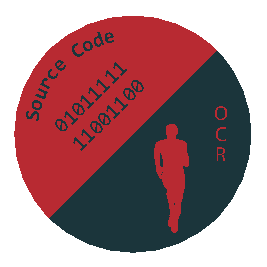
\includegraphics[width=0.3\textwidth]{images/logo.pdf}
\caption{Grafik-Bsp}
\label{fig:Grafik-Bsp}%% anpassen
\end{figure}

\lstset{language=TeX}% C, TeX, Bash, Python 
\begin{lstlisting}[
	%caption={}, label={code:}%% anpassen
]
![Grafik-Bsp](images/logo.pdf){width=30%}
\end{lstlisting}

Abbildung-Bsp vgl.~(\autoref{fig:Abbildung-Bsp}).

\begin{figure}[!ht]% hier: !ht
\centering
\includegraphics[width=0.6\textwidth]{images/Chili-1.pdf}
\caption{Abbildung-Bsp}
\label{fig:Abbildung-Bsp}%% anpassen
\end{figure}

\lstset{language=TeX}% C, TeX, Bash, Python 
\begin{lstlisting}[
	%caption={}, label={code:}%% anpassen
]
![Abbildung-Bsp](images/Chili-1.pdf){width=60%}
\end{lstlisting}

\section{Tabelle}\label{tabelle}

Tabelle-Bsp vgl.~(\autoref{tab:Tabelle-Bsp}).

\begin{table}[!ht]% hier: !ht 
\centering 
	\caption{Tabelle-Bsp} \label{tab:Tabelle-Bsp}%% anpassen 
\begin{tabular}{@{}rll@{}}
\hline
\textbf{Nr.} & \textbf{Begriffe} & \textbf{Erklärung} \\ 
\hline
1 & a1 & a2 \\ 
2 & b1 & b2 \\ 
3 & c1 & c2 \\ 
4 & a1 & a2 \\ 
\hline
\end{tabular} 
\end{table}

\lstset{language=TeX}% C, TeX, Bash, Python 
\begin{lstlisting}[
	%caption={}, label={code:}%% anpassen
]
| **Nr.** | **Begriffe** | **Erklärung** |
| ------: | :----------- | :------------ |
|       1 | a1           | a2            |
|       2 | b1           | b2            |
|       3 | c1           | c2            |
|       4 | a1           | a2            |
\end{lstlisting}

\section{Mathematik}\label{mathematik}

$[V] = [\Omega] \cdot [A]$ o. $U = R \cdot I$ o. $R = \frac{U}{I}$

\lstset{language=TeX}% C, TeX, Bash, Python 
\begin{lstlisting}[
	%caption={}, label={code:}%% anpassen
]
$[ V ] = [ \Omega ] \cdot [ A ]$ o. $U = R \cdot I$ o. $R = \frac{U}{I}$
\end{lstlisting}

$5~cm$, $a \cdot b$, $\cdots$, $\Omega$

$100^\circ\text{C}$

$80~\%$

\lstset{language=TeX}% C, TeX, Bash, Python 
\begin{lstlisting}[
	%caption={}, label={code:}%% anpassen
]
$5~cm$, $a \cdot b$, $\cdots$, $\Omega$
$100^\circ\text{C}$  
// ACHTUNG: Prozentzeichen macht Probleme in HTML und Latex 
// Z.B. 80 %
$80~\%$ // in Latex
$80~%$  // in HTML
\end{lstlisting}

\textbf{Mathematik-Umgebung}

\begin{equation}
  \sum_{i=1}^5 a_i = a_1 + a_2 + a_3 + a_4 + a_5
\end{equation}

\begin{align*}
    \sum_{i=1}^5 a_i = a_1 + a_2 + a_3 + a_4 + a_5
\end{align*}

\lstset{language=TeX}% C, TeX, Bash, Python 
\begin{lstlisting}[
	%caption={}, label={code:}%% anpassen
]
\begin{align*}
    \sum_{i=1}^5 a_i = a_1 + a_2 + a_3 + a_4 + a_5
\end{align*}
\end{lstlisting}

\section{Texthervorhebung}\label{texthervorhebung}

\textbf{Fett} oder \emph{Kursiv}

\lstset{language=TeX}% C, TeX, Bash, Python 
\begin{lstlisting}[
	%caption={}, label={code:}%% anpassen
]
**Fett** oder *Kursiv*
\end{lstlisting}

\section{Code}\label{code}

Hallo Welt vgl.~(\autoref{code:HalloWelt}).

\lstset{language=C}% C, TeX, Bash, Python 
\begin{lstlisting}[
	caption={Hallo Welt}, label={code:HalloWelt}%% anpassen
]
// hallowelt.c
#include <stdio.h>
int main(void) {
    printf("Hallo Welt!\n");
    return 0;
}
\end{lstlisting}

\section{Links}\label{links}

\url{https://google.de} oder \href{https://google.de}{Google}

\lstset{language=TeX}% C, TeX, Bash, Python 
\begin{lstlisting}[
	%caption={}, label={code:}%% anpassen
]
<https://google.de> oder [Google](https://google.de)
\end{lstlisting}

Fußnote\footnote{\url{https://bw-ju.de/}}

\lstset{language=TeX}% C, TeX, Bash, Python 
\begin{lstlisting}[
	%caption={}, label={code:}%% anpassen
]
Fußnote[^1]       

[^1]: <https://bw-ju.de/>
\end{lstlisting}

\section{Absätze}\label{absaetze}

Dies hier ist ein Blindtext zum Testen von Textausgaben. Wer diesen Text
liest, ist selbst schuld. Der Text gibt lediglich den Grauwert der
Schrift an. Ist das wirklich so? Ist es gleichgültig, ob ich schreibe:
>>Dies ist ein Blindtext<< oder >>Huardest gefburn<<? Kjift -
mitnichten! Ein Blindtext bietet mir wichtige Informationen. An ihm
messe ich die Lesbarkeit einer Schrift, ihre Anmutung, wie harmonisch
die Figuren zueinander stehen und prüfe, wie breit oder schmal sie
läuft. Ein Blindtext sollte möglichst viele verschiedene Buchstaben
enthalten und in der Originalsprache gesetzt sein. Er muss keinen Sinn
ergeben, sollte aber lesbar sein.

Fremdsprachige Texte wie >>Lorem ipsum<< dienen nicht dem eigentlichen
Zweck, da sie eine falsche Anmutung vermitteln.
 % example
	%\chapter{Schreiben in Markdown}\label{schreiben-in-markdown}

\begin{enumerate}
\item
  Markdown
\item
  Textauszeichnung -- Was ist wichtig? Tabellen, Bilder, Quellcode,
  Literatur, Links
\item
  Rechtschreibprüfung \footnote{\url{https://languagetoolplus.com/?pk-campaign=addon2-popup-logo}}
\item
  Literatur \footnote{\url{https://www.zotero.org/user/login}}
\end{enumerate}

\section{Markdown -- Latex -- PDF
erstellen}\label{markdown-latex-pdf-erstellen}

\begin{enumerate}
\item
  Markdown > Latex: \verb|$ projekt.sh|
  Script (pandoc)
\item
  Hand-Kopie: \verb|tex\_pandoc/ tex/|
\item
  Referenzen: Links prüfen

  \begin{itemize}
  \item
    Bild %vgl.~(\autoref{fig:}). >
    \verb|(\\autoref\{fig:bild\}).|
  \item
    Tabelle %vgl.~(\autoref{tab:}). >
    \verb|(\\autoref\{tab:tabellen\}).|
  \item
    Kapitel %vgl.~(\autoref{}). >
    \verb|(\\autoref\{sec:zusammenfassung\}).|
  \item
    Code %vgl.~(\autoref{code:}). >
    \verb|(\\autoref\{code:hallowelt\})|.
  \end{itemize}
\item
  Latex > PDF: \verb|$ make| Makefile
  (latexmk)
\end{enumerate}

\section{Quellen}\label{quellen}

Quelle: \textcite{spanner:2019:robotik} 

Quelle: \textcite{homofaciens:2018:projekt}

Quelle: \textcite{kofler:2018:hacking}

\lstset{language=TeX}% C, TeX, Bash, Python 
\begin{lstlisting}[
	%caption={}, label={code:}%% anpassen
]
Quelle: [@monk:2016:action]
Quelle: [@homofaciens:2018:projekt]
Quelle: [@kofler:2018:hacking]
\end{lstlisting}

\section{Listen}\label{listen}

\textbf{ungeordnete Liste}

\begin{itemize}
\item
  a
\item
  b

  \begin{itemize}
  \item
    BB
  \end{itemize}
\item
  c
\end{itemize}

\lstset{language=TeX}% C, TeX, Bash, Python 
\begin{lstlisting}[
	%caption={}, label={code:}%% anpassen
]
- a
- b
    - bb
- c
\end{lstlisting}

\textbf{Sortierte Liste}

\begin{enumerate}
\item
  eins
\item
  zwei
\item
  drei
\end{enumerate}

\lstset{language=TeX}% C, TeX, Bash, Python 
\begin{lstlisting}[
	%caption={}, label={code:}%% anpassen
]
1. eins
2. zwei
3. drei
\end{lstlisting}

\textbf{Sortierte Liste}

\begin{enumerate}
\def\labelenumi{\alph{enumi})}
\item
  a
\item
  b
\item
  c
\end{enumerate}

\lstset{language=TeX}% C, TeX, Bash, Python 
\begin{lstlisting}[
	%caption={}, label={code:}%% anpassen
]
a) a
b) b
c) c
\end{lstlisting}

\section{Anführungszeichen}\label{anfuehrungszeichen}

>>Anführungszeichen<<

\lstset{language=TeX}% C, TeX, Bash, Python 
\begin{lstlisting}[
	%caption={}, label={code:}%% anpassen
]
"Anführungszeichen" 
\end{lstlisting}

\section{Grafik und Abbildung}\label{grafik-abbildung}

Grafik-Bsp vgl.~(\autoref{fig:Grafik-Bsp}).

\begin{figure}[!ht]% hier: !ht
\centering
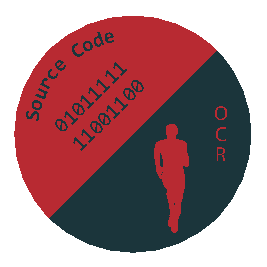
\includegraphics[width=0.3\textwidth]{images/logo.pdf}
\caption{Grafik-Bsp}
\label{fig:Grafik-Bsp}%% anpassen
\end{figure}

\lstset{language=TeX}% C, TeX, Bash, Python 
\begin{lstlisting}[
	%caption={}, label={code:}%% anpassen
]
![Grafik-Bsp](images/logo.pdf){width=30%}
\end{lstlisting}

Abbildung-Bsp vgl.~(\autoref{fig:Abbildung-Bsp}).

\begin{figure}[!ht]% hier: !ht
\centering
\includegraphics[width=0.6\textwidth]{images/Chili-1.pdf}
\caption{Abbildung-Bsp}
\label{fig:Abbildung-Bsp}%% anpassen
\end{figure}

\lstset{language=TeX}% C, TeX, Bash, Python 
\begin{lstlisting}[
	%caption={}, label={code:}%% anpassen
]
![Abbildung-Bsp](images/Chili-1.pdf){width=60%}
\end{lstlisting}

\section{Tabelle}\label{tabelle}

Tabelle-Bsp vgl.~(\autoref{tab:Tabelle-Bsp}).

\begin{table}[!ht]% hier: !ht 
\centering 
	\caption{Tabelle-Bsp} \label{tab:Tabelle-Bsp}%% anpassen 
\begin{tabular}{@{}rll@{}}
\hline
\textbf{Nr.} & \textbf{Begriffe} & \textbf{Erklärung} \\ 
\hline
1 & a1 & a2 \\ 
2 & b1 & b2 \\ 
3 & c1 & c2 \\ 
4 & a1 & a2 \\ 
\hline
\end{tabular} 
\end{table}

\lstset{language=TeX}% C, TeX, Bash, Python 
\begin{lstlisting}[
	%caption={}, label={code:}%% anpassen
]
| **Nr.** | **Begriffe** | **Erklärung** |
| ------: | :----------- | :------------ |
|       1 | a1           | a2            |
|       2 | b1           | b2            |
|       3 | c1           | c2            |
|       4 | a1           | a2            |
\end{lstlisting}

\section{Mathematik}\label{mathematik}

$[V] = [\Omega] \cdot [A]$ o. $U = R \cdot I$ o. $R = \frac{U}{I}$

\lstset{language=TeX}% C, TeX, Bash, Python 
\begin{lstlisting}[
	%caption={}, label={code:}%% anpassen
]
$[ V ] = [ \Omega ] \cdot [ A ]$ o. $U = R \cdot I$ o. $R = \frac{U}{I}$
\end{lstlisting}

$5~cm$, $a \cdot b$, $\cdots$, $\Omega$

$100^\circ\text{C}$

$80~\%$

\lstset{language=TeX}% C, TeX, Bash, Python 
\begin{lstlisting}[
	%caption={}, label={code:}%% anpassen
]
$5~cm$, $a \cdot b$, $\cdots$, $\Omega$
$100^\circ\text{C}$  
// ACHTUNG: Prozentzeichen macht Probleme in HTML und Latex 
// Z.B. 80 %
$80~\%$ // in Latex
$80~%$  // in HTML
\end{lstlisting}

\textbf{Mathematik-Umgebung}

\begin{equation}
  \sum_{i=1}^5 a_i = a_1 + a_2 + a_3 + a_4 + a_5
\end{equation}

\begin{align*}
    \sum_{i=1}^5 a_i = a_1 + a_2 + a_3 + a_4 + a_5
\end{align*}

\lstset{language=TeX}% C, TeX, Bash, Python 
\begin{lstlisting}[
	%caption={}, label={code:}%% anpassen
]
\begin{align*}
    \sum_{i=1}^5 a_i = a_1 + a_2 + a_3 + a_4 + a_5
\end{align*}
\end{lstlisting}

\section{Texthervorhebung}\label{texthervorhebung}

\textbf{Fett} oder \emph{Kursiv}

\lstset{language=TeX}% C, TeX, Bash, Python 
\begin{lstlisting}[
	%caption={}, label={code:}%% anpassen
]
**Fett** oder *Kursiv*
\end{lstlisting}

\section{Code}\label{code}

Hallo Welt vgl.~(\autoref{code:HalloWelt}).

\lstset{language=C}% C, TeX, Bash, Python 
\begin{lstlisting}[
	caption={Hallo Welt}, label={code:HalloWelt}%% anpassen
]
// hallowelt.c
#include <stdio.h>
int main(void) {
    printf("Hallo Welt!\n");
    return 0;
}
\end{lstlisting}

\section{Links}\label{links}

\url{https://google.de} oder \href{https://google.de}{Google}

\lstset{language=TeX}% C, TeX, Bash, Python 
\begin{lstlisting}[
	%caption={}, label={code:}%% anpassen
]
<https://google.de> oder [Google](https://google.de)
\end{lstlisting}

Fußnote\footnote{\url{https://bw-ju.de/}}

\lstset{language=TeX}% C, TeX, Bash, Python 
\begin{lstlisting}[
	%caption={}, label={code:}%% anpassen
]
Fußnote[^1]       

[^1]: <https://bw-ju.de/>
\end{lstlisting}

\section{Absätze}\label{absaetze}

Dies hier ist ein Blindtext zum Testen von Textausgaben. Wer diesen Text
liest, ist selbst schuld. Der Text gibt lediglich den Grauwert der
Schrift an. Ist das wirklich so? Ist es gleichgültig, ob ich schreibe:
>>Dies ist ein Blindtext<< oder >>Huardest gefburn<<? Kjift -
mitnichten! Ein Blindtext bietet mir wichtige Informationen. An ihm
messe ich die Lesbarkeit einer Schrift, ihre Anmutung, wie harmonisch
die Figuren zueinander stehen und prüfe, wie breit oder schmal sie
läuft. Ein Blindtext sollte möglichst viele verschiedene Buchstaben
enthalten und in der Originalsprache gesetzt sein. Er muss keinen Sinn
ergeben, sollte aber lesbar sein.

Fremdsprachige Texte wie >>Lorem ipsum<< dienen nicht dem eigentlichen
Zweck, da sie eine falsche Anmutung vermitteln.
  
	%%ju 22-Jul-21 Neu.tex
Neuer Inhalt
 % neu

	% Bibliographie
	\ifisbook\cleardoubleemptypage\fi
	\phantomsection\addcontentsline{toc}{chapter}{\refname}
	\printbibliography
	
\end{document}